\documentclass{article}
\usepackage{graphicx,fancyhdr,amsmath,amssymb,amsthm,subfig,url,hyperref}
\usepackage[margin=1in]{geometry}

\usepackage{natbib}
\usepackage{cancel}

\usepackage{minted}

\usepackage[shortlabels]{enumitem}

%----------------------- Macros and Definitions --------------------------

%%% FILL THIS OUT
\newcommand{\studentname}{Jane Doe}
\newcommand{\suid}{janedoe}
\newcommand{\exerciseset}{Homework}
%%% END



\renewcommand{\theenumi}{\bf \Alph{enumi}}

\theoremstyle{plain}
\newtheorem{theorem}{Theorem}
\newtheorem{lemma}[theorem]{Lemma}


\graphicspath{{figures/}}

%-------------------------------- Title ----------------------------------

\title{Study Kasus 2: \textit{Cobweb} dalam Bidang Ekonomi} 
\author{IN232 Matematika Diskrit}
\date{}
%--------------------------------- Text ----------------------------------

\begin{document}
\maketitle

%	\begin{enumerate}[-,topsep=0pt, nosep,label=\alph*. ]
%		\item How many ways are there to pick two representatives, so that one is a mathematics major and the other is a computer science major?
%		\item How many ways are there to pick one representative who is either a mathematics major or a computer science major?
%	\end{enumerate}

\section*{Latar Belakang}
\begin{figure}[!ht]
	\centering
	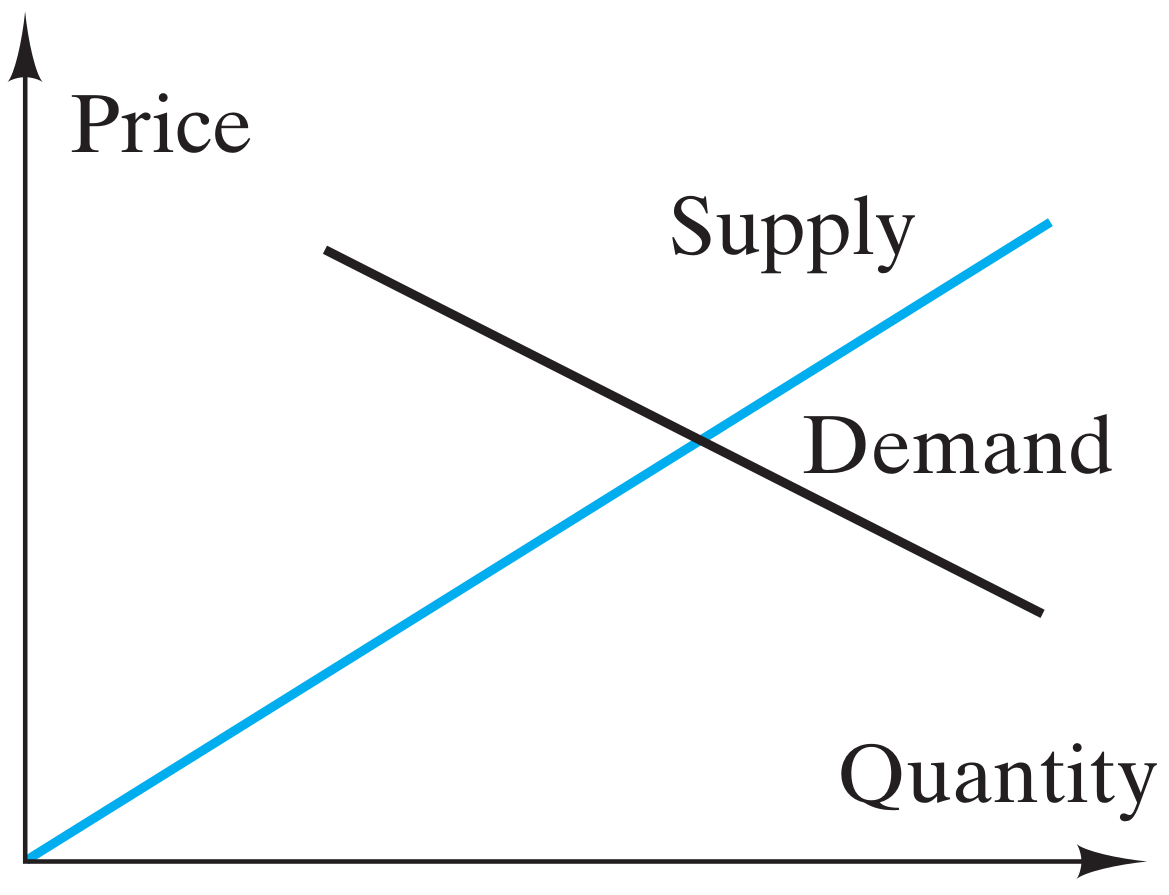
\includegraphics[scale=.15]{images/model-ekonomi}
	\caption{Model ekonomi dengan dua garis lurus sebagai penawaran (\textit{supply}) dan permintaan (\textit{demand}) \citep{johnsonbaugh2009discrete}}
	\label{fig:model-ekonomi}
\end{figure}
\noindent Asumsikan bahwa model ekonomi memiliki penawaran (\textit{supply}) dan permintaan (\textit{demand}) yang diberikan oleh dua persamaan linier pada Figure \ref{fig:model-ekonomi}. Persamaan \textit{demand} diberikan oleh persamaan 
\begin{equation}
	p = a - bq,
	\label{eq:demand-equation}
\end{equation}
dengan $p$ adalah harga (\textit{price}), $q$ adalah kuantitas atau jumlah (\textit{quantity}), dan $a$ dan $b$ adalah masing-masing parameter bernilai positif. Idenya adalah bahwa ketika harga (\textit{price}) meningkat, permintaan konsumen menurun. Persamaan \textit{supply} digambarkan oleh persamaan
\begin{equation}
	p = kq,
\end{equation}
dengan $p$ adalah harga (\textit{price}), $q$ adalah kuantitas atau jumlah (\textit{quantity}), dan $k$ adalah parameter bernilai positif.

Asumsikan lebih lanjut bahwa ada jeda waktu ketika penawaran bereaksi terhadap perubahan. (Sebagai contoh, waktu dibutuhkan untuk memproduksi barang dan juga waktu dibutuhkan untuk bercocok tanam.) Interval waktu diskrit ditunjukkan sebagai $n = 0,1, \ldots$. Dengan adanya interval waktu diskrit ini, asumsikan bahwa \textit{demand} digambarkan oleh 

\begin{equation}
	p_n = a - bq_n,
	\label{eq:demand-equation-time}
\end{equation}

\noindent dengan pada saat waktu $n$, kuantitas $q_n$ dari suatu produk akan dijual pada harga $p_n$. Demikian juga dengan asumsi \textit{supply} diberikan oleh

\begin{equation}
	p_n = kq_{n+1},
	\label{eq:supply-equation-time}
\end{equation}

\noindent dengan satu unit waktu diperlukan bagi pabrikan untuk memproduksi produk dengan kuantitas $q_{n+1}$, pada waktu $n + 1$, dengan harga $p_n$, pada waktu sebelumnya, yaitu $n$. Persamaan \eqref{eq:supply-equation-time} dapat ditulis sebagai 

\begin{equation}
	q_{n+1} = p_n / k.
	\label{eq:supply-equation-time-alternative}
\end{equation}

Dengan menuliskan Persamaan \eqref{eq:demand-equation-time} pada saat $n+1$, yaitu $p_{n+1} = a - b q_{n+1}$ dan melakukan substitusi Persamaan \eqref{eq:supply-equation-time-alternative} ke dalamnya, diperoleh relasi rekurensi dari \textit{price} sebagai berikut:

\begin{equation}
	p_{n+1} = a - \frac{b}{k} p_n
	\label{eq:price-recursive-relation}
\end{equation}

Perubahan harga sepanjang waktu dapat dilihat secara grafis. Jika harga awalnya adalah $p_0$, pabrikan akan bersedia menyediakan kuantitas $q_1$, pada waktu $n = 1$. Kuantitas ini ditemukan dengan bergerak secara horizontal ke kurva \textit{supply} (lihat Figure \eqref{eq:cobweb-ilustrasi}). Namun, kekuatan pasar mendorong harga turun ke $p_1$, seperti yang dapat dilihat ketika terjadi pergerakan vertikal ke kurva \textit{demand}. Pada harga $p_1$, pabrikan akan bersedia menyediakan jumlah $q_2$ pada waktu $n = 2$, seperti yang diperlihatkan ketika terjadi pergerakan secara horizontal ke kurva \textit{supply}. Sekarang kekuatan pasar mendorong harga hingga $p_2$, seperti yang terlihat dengan pergerakan secara vertikal ke kurva \textit{demand}.
Dengan melanjutkan proses ini, "sarang laba-laba" diperoleh seperti yang ditunjukkan pada Figure \eqref{eq:cobweb-ilustrasi}.

\begin{figure}[!ht]
	\centering
	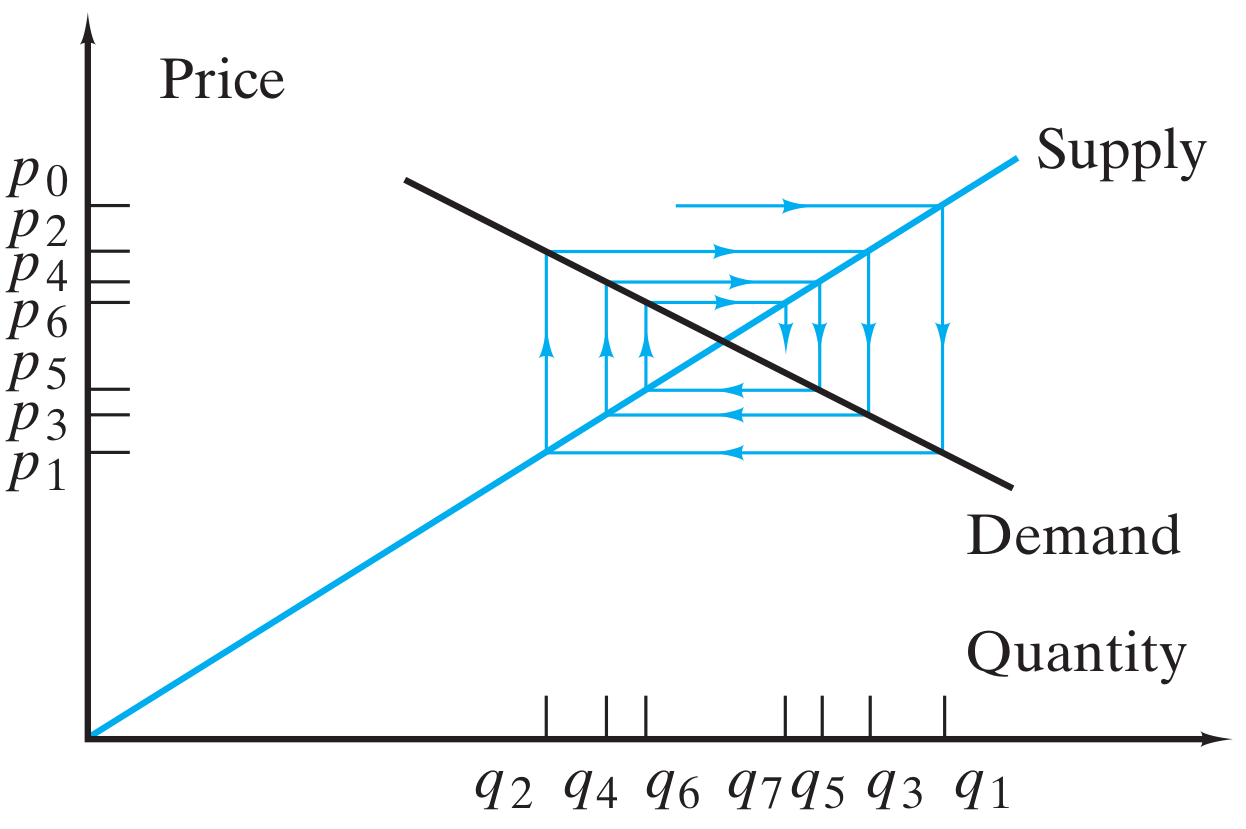
\includegraphics[scale=.225]{images/cobweb-ilustrasi}
	\caption{Cobweb dengan harga yang stabil \citep{johnsonbaugh2009discrete}}
	\label{eq:cobweb-ilustrasi}
\end{figure}

\section*{Implementasi}
	\begin{enumerate}[-,topsep=0pt, nosep,label=\arabic*. ]
		\item Ubahlah relasi rekurensi di Persamaan \eqref{eq:price-recursive-relation} menjadi \textit{solusi eksplisit}.  
		\item Implementasi Persamaan \eqref{eq:price-recursive-relation} dalam program.
	\end{enumerate}

\begin{minted}{python}
def compute_cobweb(p_0, a, b, k, n):
    """
    Compute a price at n based on cobweb recursive relation	
    
    Parameters:
    -----------
    p_0 : float
        An initial price
    
    a, b, k : float
        Three positive parameters
    
    n : int
        The final time for the price to be computed    
    
    Returns:
    --------
    p_n : float
        The final price at time n
    """
    pass
\end{minted}

\noindent Sebagai test drive, silakan anda hitung secara manual dan bandingkan hasil manual dengan hasil program.


\bibliographystyle{apalike}
\bibliography{references}


\end{document}
